\documentclass[12pt,a4paper]{article} % document setting, articles do not allow chapters
\usepackage[english]{babel} % english spell-check
\usepackage[utf8]{inputenc} % allows the input of special characters from keyboard
\usepackage[T1]{fontenc}
\usepackage{lmodern} %load modern fonts
\usepackage{helvet} % lead helvetica font
\renewcommand{\familydefault}{\sfdefault} % without this helvetica does not work on linux
\usepackage{textcomp} % for text symbols such as (C)
\usepackage{siunitx} % for mathematical embedding with $

\AtBeginDocument{\renewcommand{\bibname}{References}} % change Bibliography to Reference in TOC
\usepackage[compress]{natbib} % include bibliography
%super, numbers
\bibliographystyle{apalike} % simple bibliography style % sudo texhash
%\bibliographystyle{plainnat} %order by appearance: unsrtnat
\usepackage{hyperref} % allow printing URLs (here: for Bibliography)
\usepackage{cite}

\usepackage{graphicx} % include figures
\usepackage[labelfont=bf]{caption} % change figure caption to bold

\usepackage{titlesec} %change title style
\titleformat*{\section}{\normalsize\bfseries}
\titleformat*{\subsection}{\normalsize\itshape}

%\usepackage[mathlines]{lineno} % add line numbers
\usepackage{setspace} %for double spacing

\author{Masumi Stadler}
\title{PhD proposal}

%%%%%%%%%%%%
% Document %
%%%%%%%%%%%%
\begin{document}
%\linenumbers

\setlength{\parindent}{0cm}
Title (max 150 char): Diverging DNA and RNA communities along a boreal terrestrial-hydrological continuum (?) \\

Masumi Stadler\textsuperscript{1,*}, Paul A. del Giorgio\textsuperscript{1}\\

Affilitation:\\
(1) Groupe de Recherche Interuniversitaire en Limnologie (GRIL), Département des Sciences Biologiques, Université du Québec à Montréal, Montréal, QC, Canada


Institutional e-mail addresses: MS (stadler.masumi@courrier.uqam.ca), PdG (del\_giorgio.paul@uqam.ca)\\

Running title (max 50 char): Microbial communities along a boreal terrestrial-hydrological continuum.\\

*Contact corresponding author: Masumi Stadler \\
E-mail: m.stadler.jp.at@gmail.com \\
Phone: +1 (514)297-5330 \\
Address: Département des Sciences Biologiques, Université du Québec à Montréal, Case Postale 8888, Succursale Centre-Ville, Montréal, QC, H3C 3P8, Canada \\

Keywords: aquatic bacterial communities, terrestrial-aquatic continuum, ecosystem connectivity, residence time, boreal ecosystems, mass effects, environmental sorting, metacommunity, rare biosphere\\

Author contributions: PdG designed the sampling, MS collected the data, MS analysed the data, MS and PdG discussed the results and wrote the manuscript.\\

\newpage

\doublespacing

%\begin{abstract}


%\end{abstract}


\setlength{\parindent}{1cm}
\section*{Introduction}
Since the 1880s, we are starting to grasp the intriguing variety of microbial physiological pathways and how they are involved in global elemental cycling \citep{Caumette2015}. Such variety in physiological pathways has been hypothesised to arise from the widely observed vast taxonomic diversity, however, little do we understand how microbes assemble into diverse communities (Shade, 2018). Microbial communities found outside of the petri-dish are inherently taxonomically diverse, with richness estimations that defy
imagination (Thompson et al., 2017). Richness varies among ecosystems with highest taxonomic reservoirs found in soil and less so in nutrient depleted aquatic ecosystems (xx,xx). Traditionally, microbial ecology has focused on one ecosystem at a time. Investigating the intriguing seasonal and spatial fluctuations of community composition within soil and aquatic ecosystems (xx). Even among freshwater studies, researchers tend to focus on streams, lakes, or rivers at a time (xx,xx,xx). While this approach gives an in-detail insight into ecosystem specific functioning, it neglects an inherent characteristic of nature: connectivity beyond ecosystem boundaries. 

Even when we study seemingly stationary organisms, the miniscule size of microorganisms promotes dispersal through wind and water (xx,xx). Thus, freshwaters act as a carrier of matter, from the terrestrial milieu over freshwater networks to ultimately the ocean. Especially during rain events, freshwater flushes through the earth, extracting all soluble nutrients and capturing matter - dead or alive - along its hydrological evolution from a raindrop to collectively becoming a stream. On its further journey, the rushing water may be stopped by lakes and reservoirs that temporarily give more time for some organisms to thrive (xx). Through the aquatic network, dynamics in hydrology have been determined to be one of the major drivers of microbial community composition (xx). This hydrological funnel collects taxa from all sub-catchments within a watershed, creating a watershed specific unique community (xx). Thus, not every member within diverse communities at a single location shares a similar history in terms of origin \citep{Nino-Garcia2016, Comte2017} or reacts similarly to changing environmental conditions \citep{Fierer2007}. However, such passive dispersal implies that occurence of a taxon in an unsuitable habitat merely by accident is indeed likely. Death and dormancy questions the suitability of DNA approaches to study ecological "communities". In a strict sense, a community refers to an assemblage of various species that interact with each other (xx). However, DNA methods are not able to distinguish the actively participating from the passive members. Recently, researchers have expanded their molecular toolbox to RNA approaches that capture taxa that have invested in cellular growth in the recent minutes to hours (xx).

As a result, recent evidence indicates that sub-groups within a community (e.g. rare versus abundant taxa) are governed by differing assembly processes \citep{Bell2000, Magurran2003}. Microbial communities are not only selected by environmental variables but also assemble stochastically to a large extent \citep{Zhou2017, Jia2018}. 




Especially in aquatic systems, where one of the main drivers of community composition has been attributed to hydrology (xx), hydrological connectivity promotes passive dispersal from sub-catchments into the freshwater network. 

The consecutive flooding of the reservoirs creates a unique opportunity to study the transformation process of a running system into a standing water body. The shifts mainly imposed due to the increased residence times are likely to influence not only biogeochemical properties but also their microbial assemblages.

(should be around 900~1000 words)

\section*{Material and methods}
\subsection*{Catchment characteristics and sampling design}
To follow the movement of microbial communities within a watershed, samples were taken along the Romaine river (C\^{o}te-Nord region, Qu\'{e}bec, Canada) (Fig. 1a-b) for three years from 2015-2017. The Romaine catchment belongs to the eastern black spruce-moss bioclimatic domain and drains an area (\textit{A}) of approximately 14 500 km\textsuperscript{2}. The catchment was glaciated 7 000 – 10 000 years ago and left mostly a till blanket and veneer as surficial material. It is mainly dominated by acid rocks (e.g. granodiorite, granite, quart diorite) with granitised sedimentary and volcanic rock, and has isolated patches of permafrost (0-10\%)(Natural Resources Canada). The soil is composed of roughly 61.4\% sand, 31.9\% silt, 6.7\% clay and stores approximately 140.4 t ha\textsuperscript{-1} of organic carbon (in top 5 cm; given are catchment averages)\citep{Lehner2013, Hengl2014}.

The river springs between the Atlantic and Saint Lawrence watersheds (52\textdegree{}52'20"N 63\textdegree{}36'55"W; 702 masl), and consequently flows through a series of lakes (hereafter riverine lakes) including the biggest lake in the catchment – Lake Br\^{u}l\'{e} (\textit{A}: 127.11 km\textsuperscript{2}, elevation: 470 masl). The river mainly flows towards the South with a maximum distance from the northern headwaters to the river mouth expanding to approximately 475.1 km. Nearly half of the catchment is covered by coniferous forests (\textit{P.mariana}-moss), with mixed forests being rather minor (11\%) and deciduous stands with white birch (\textit{Betula papyrifera}) and trembling aspen (\textit{Populus tremuloides}) are even more rare (2\%)\citep{HQreport2009}. The northern part of the catchment is characterised by a flat open black spruce (\textit{Picea mariana})-lichen forest with shrubs and moss-lichen (Fig. S1a). As one follows the river downstream, the relief changes drastically to a steep mountainous stretch that forms sections of canyons (Fig. S1b). The river looses 330 m of elevation from the mountainous section until it makes a sharp turn to the west into the lower coastal plain. The coastal plain is characterised by peatland areas with swamps and shallow waters that are completely permafrost free (Fig. S1c). There are two larger tributaries in the coastal plain that flow through the lakes Puyjalon (\textit{A}: 13.10 km\textsuperscript{2}) and Allard (\textit{A}: 19.24 km\textsuperscript{2}). A weather station located in the lower coastal plain (50\textdegree{} 16'55.000" N, 63\textdegree{} 36'41.000" W, Havre-Saint-Pierre Airport, Natural Resources Canada) recorded an annual precipitation of 810.77 $\pm$ 35.25 mm and 1.18 $\pm$ 0.73 \textdegree{}C, -32.63 $\pm$ 1.36 \textdegree{}C, and 25.8 $\pm$ 0.66 \textdegree{}C for mean, minimum and maximum temperature over the sampled years. 

The Romaine river has been dammed during the sampling period, forming a reservoir cascade complex with 4 reservoirs by 2020. The reservoirs Romaine 2 (RO2, \textit{A}: 81.15 km\textsuperscript{2}, mean depth 61 m), Romaine 1 (RO1, \textit{A}: 13.22 km\textsuperscript{2}, mean depth 22 m) and Romaine 3 (RO3, \textit{A}: 35.18 km\textsuperscript{2}, mean depth 66 m) were flooded in the years 2014 (winter), 2015 (winter), and 2017 (spring), respectively.

Overall, 395 samples were collected for DNA (D) and 202 for RNA (R), covering spring (166-D, 69-R), summer (195-D, 99-R) and autumn (34-D, 34-R). RNA samples were sampled from 2016 onwards. To follow a terrestrial-aquatic continuum various habitat types have been sampled (Table S1). Due to the remoteness and inaccessibility of the northern most headwaters, we have sampled the Petite Romaine sub-catchment (PR, \textit{A}: 310.73 km\textsuperscript{2}, elevation: 580 masl, Fig. 1c) for streams and headwater ponds. This sub-catchment represents a headwater stream network in our studied continuum. 

Surface soil samples were collected by mixing three randomly selected cores (30 cm) that were taken in proximity of installed piezometers to sample soil-water. The upper 5 cm including surface vegetation were removed before the soil was transferred into a sterile plastic bag. Three piezometers were randomly installed in proximity (30-100 cm) to a sampled stream with an average depth of 50 $\pm$ 20 cm. However, if the piezometers were installed too close to the stream main channel, hyporheic water was sampled instead. Piezometers were emptied 3 times (1-2 h) with a peristaltic pump before sample water was collected. The water from the randomly installed piezometers were pooled together. Groundwater was direcy collected from constructed wells with submersible pumps. Surface water samples were directly collected into a pre-rinsed carboy bottle at a depth of 0.5 m, close to the shore for stream samples and diverse locations within the river and reservoirs. Lake sediment samples were collected with sediment cores (1-2 m depth), and the upper 10 cm were collected and mixed for subsequent processing. All samples were stored at 4 \textdegree{}C upon arrival at the laboratory until further processing on the same day of sampling. 

\subsection*{Sample processing and sequencing}
Homogenised soil and sediment samples were transferred to aliquots of 0.25 g and frozen immediately on the same day of sampling. A minimum of 25 mL and 250 mL of soil-/hyporheic-water and surface water was filtered through 0.22 \si\micro m polycarbonate membrane filters (Merck Millipore, Darmstadt, Germany), respectively, and subsequently stored frozen. All DNA and RNA samples were frozen at -20 \textdegree{}C at the field station and further stored at -80 \textdegree{}C at the university laboratory until extraction. Samples for RNA extraction were submerged in RNAlater\textsuperscript{\textregistered} and LifeGuard\textsuperscript{\textregistered} Soil Preservation solution (QIAGEN\textsuperscript{\textregistered}, Hilden, Germany) for water and humic samples (soil, soilwater, hyporheic water), respectively. To allow stabilisation, samples were left at 4 \textdegree{}C overnight and were subsequently stored frozen.

Following the manufacturers instructions, PowerWater\textsuperscript{\textregistered} and PowerSoil\textsuperscript{\textregistered} DNA and RNA extraction kits (MoBio, Carlsbad, CA, USA) were used to extract water and soil/soil-/hyporheic-water/sediment samples, respectively. In 2017, the equivalent DNeasy\textsuperscript{\textregistered} and RNeasy\textsuperscript{\textregistered} PowerWater\textsuperscript{\textregistered} Kits (QIAGEN\textsuperscript{\textregistered}) were used for DNA and RNA samples, respectively. cDNA was synthesised from the extracted RNA with a high capacity cDNA Reverse Transcription Kit (Applied Biosystems\textsuperscript{\texttrademark}, Foster City, CA, USA). Successful extraction was evaluated via PCR amplification of the 515F-806R primers (IDT Technologies, Coralville, IA, USA) and DNA concentration was measured with a NanoDrop 2000c (Thermo Fisher Scientific Inc., Waltham, MA, USA). Extracts were sent to G\'{e}nome Qu\'{e}bec Innovation Centre (Montr\'{e}al, QC, Canada) for paired-end metabarcoding of the 16S rRNA V4 region using the primers 515F (5'-GTGCCAGCMGCCGCGGTAA-3') and 806R (5'-GGACTACHVGGGTWTCTAAT-3') on a Illumina MiSeq (PE250) platform.

\subsection*{Bioinformatic analysis}
Primers were removed using the software \textit{cutadapt} (Version 1.18, \citet{Martin2013}), which allows for the removal of the primer sequence and its variants in their true and complement orientations. Additionally, all reads shorter than 125 nucleotides were removed as they cannot achieve a minimum overlap necessary for paired-end merging in downstream processing.

To identify amplicon sequence variants (ASVs), 16S rRNA amplicon reads were analysed through the DADA2 (Divisive Amplicon Denoising Algorithm 2) pipeline (Version 1.14.1, \citet{Callahan2017}) on R Version 3.6.3 \citep{RCoreTeam2017}). Read qualities were evaluated for each sequencing plate separately and read length was trimmed according to their quality scores. The most conservative trimming criteria still allowed for an overlap of forward and reverse reads by 60 bp. Samples were pooled by plate, season and sequencing depth for learning the error rates. DADA2 runs on a sample by sample basis, and thus removes observed singletons by sample to avoid inclusion of false-positive sequencing errors. To retain more rare taxa within a sampling campaign (year-season combinations) along the continuum, samples were 'pseudo'-pooled for the \textit{dada()} step.  This step enables the removal of singletons by pool but retains singletons within a sample. Paired-ends were merged after successful inference of amplicon variants. Subsequently, all ASVs that are identical in sequence but differ only by length were merged together with \textit{collapseNoMismatch()}, leading to ASVs that represent a unit similar to 100\% similarity operational taxonomix units (OTUs) and chimeras were removed (\textit{removeBimeraDenovo()}). Finally, taxonomy was assigned with the \textit{DECIPHER} package (Version 2.14.0, \citet{Wright2016}) implementing the increased accuracy IDTAXA algorithm \citep{Murali2018} and the provided trained classifier of the SILVA database (Version 138, \citet{Pruesse2007}). Only ASVs that were classified as Bacteria and not as Mitochondria or Chloroplast were evaluated in this study. Even after merging ASVs into 100\% OTUs, several ASVs were found to be highly abundant only in RNA. To account for slight differences that may have emerged between DNA and RNA ASVs and also to merge potential differences among 16S rRNA copies within a single genome \citep{Vetrovsky2013a}, ASVs were merged into OTUs by a 99\% similarity threshold (\textit{DECIPHER}: \textit{AlignSeqs(), DistanceMatrix(), IdClusters()}, \citet{Wright2016}). To keep computational power low, OTU clustering was conducted within taxonomical pools. Such that ASVs classified only as "Bacteria" without any classification in further ranks were pooled for clustering, while any ASV with a classifcation in any higher rank was clustered with other ASVs that had the same highest assigned taxonomical rank (e.g. "Bacteria-Proteobacteria-Gammaproteobacteria-Burkholderiales-Burkholderiaceae-Limnobacter" pool).

All OTU observations with less than 10 reads per sample were removed. Furthermore, \textit{metagenomeSeq} was used to transform and stabilise variation in library sizes with cumulative sum scaling (CSS) \citep{Paulson2013}. CSS results were rounded to its integer to represent count data (hereafter: CSS reads). CSS results were compared with results achieved with various rarefaction thresholds. To account for random sampling effects, rarefaction was conducted with 100 random iterations. Similarly to the CSS data treatments, the mean of all iterations was rounded to its integer to be used for subsequent analysis. There were no substantial differences in the results between CSS and various rarefaction thresholds (Fig. S2). Consequently, CSS results were used for downstream analyses.

\subsection*{Data handling and statistical analyses}
To explore differences in microbial community composition across habitat types and seasons, a Principal Coordinates Analysis (PCoA) was conducted with Bray-Curtis dissimilarities based on all DNA samples with the function \textit{pcoa} in the \textit{ape} package \citep{Paradis2018}) (n = 372, 20185 OTUs). The community matrix was log transformed, (log\textsubscript{2}(x + 1)) to resolve a strong horse-shoe effect. The Bray-Curtis dissimilarity matrix was square-root transformed to make the distance matrix Euclidean \citep{Legendre1998, Borcard2011}. A PERMANOVA was computed with 9999 permutations to evaluate statistical differences in habitat type and season  with the \textit{adonis} function in \textit{vegan} \citep{Oksanen2017}. The null hypothesis of this approach is that the cluster centroids do not differ between groups \citep{Anderson2013}. The test cannot distinguish among-group from within-group variation if data disperion is variable among groups. Thus, an analysis of multivariate homogeneity was computed with \textit{betadisper} in \textit{vegan} \citep{Oksanen2017} by accounting for small and uneven sample sizes with the \textit{bias.adjust} argument. Using \textit{permutest} in \textit{vegan} \citep{Oksanen2017}, we tested whether dispersion is variable among groups. The null hypothesis is that the average within-group dispersion is equivalent in all groups \citep{Anderson2013}.

Secondly, to evaluate whether sampled RNA communities were further different from the DNA assemblages, we performed a second PCoA (Bray-Curtis dissimilarities with square-root transformation) with both DNA and RNA samples (n = 572, 20220 OTUs). Again, statistically different clusters were investigated with a PERMANOVA (9999 permutations), where habitat type, season and nucleic acid type (DNA-RNA) formed the clusters. The same framework explained above to check for dispersions was applied. For all statistical analyses, an $\alpha$ level of 0.05 was chosen prior to analysis.

To examine how different DNA and RNA assemblages of the same sample are, the distance of each DNA-RNA sample pair within the PCoA ordination space was computed. Distance was calculated along the second axis, as it was identified to separate DNA and RNA within the ordination space. Summation of the distances across all PCoA dimensions (571 axes) equals the initial pair-wise Bray-Curtis dissimilarites. 

Non-linear regressions were computed to test the hypothesis that DNA-RNA distances are a function of $\alpha$ diversity indices (Shannon-Wiener index and Pielou's evenness). Regressions were computed on the means of habitat types. The best fit of the relationship was evaluated by computing linear regressions and polynomials of second and third degrees. The best model was selected based on a higher adjusted R\textsuperscript{2} and low residual sum squares.

\subsubsection*{Abundance classification}
Traditionally, abundance groups such as "abundant" and "rare" have been defined by various relative abundance thresholds ranging from 0.1 to 1 \% within the literature. While inconsistencies hinder comparisons among studies, we additionally are working with variance stabilised read numbers, thus traditional thresholds based on relative abundances are not applicable. In order to classify OTUs into abundance groups, we developed a new framework to classify OTUs into abundance groups based on the shape of rank abundance curves. We initiate the framework by calculating the mean abundance of each OTU for each habitat type. Subsequently, for each habitat type a smoothed rank abundance curve was generated with the function \textit{smooth.spline} with the smoothing parameter set to 0.7 in base R (Fig. S2a). Ranks that correspond to moments of acceleration along the curve were identified by taking the second derivative of the log(x + 1) transformed abundance curve (Fig. S2c). All OTUs ranked below the second maximum acceleration were defined as rare. OTUs falling above the first maximum acceleration were defined as abundant, while the section in between the two maxima represents moderately abundant OTUs (Fig. S2). The CSS reads corresponding to the ranks identified for each abundance group were extracted for each habitat type seperately. Subsequently, the average CSS reads for each threshold was calculated. This approach classified all OTUs with >= 47 CSS reads as abundant, < 47 and >= 5 CSS reads as moderate, and < 5 CSS reads as rare.

As the second step, we defined OTUs into spatial abundance groups based on their DNA abundances (Table xx). In brief, OTUs that are abundant, moderate or rare in all habitat types were classifed as universally abundant, moderate, and rare, respectively. However, for the category universally rare, OTUs did not have to be present in all habitat types. Any OTU that is never rare but fluctuates between abundant and moderate was classified as cosmopolitan. We further separated habitat types into three ecosystem domains: Terrestrial (soil, soilwater, groundwater and sediment), freshwater and marine. An OTU that is abundant in all samples of one ecosystem domain, but never abundant in other domains was defined as a domain specialist. Finally, four categories of shifters were defined. Where OTUs can shift between being abundant, moderate and rare. OTUs that are present in all habitat types and mostly abundant (>= 50\% of habitat types) are universal abundant shifters, while mostly rare OTUs are universal rare shifters. The last two categories capture OTUs that are absent in certain habitat types but are more frequently abundant (abundant shifter) or more frequently rare (rare shifter).

To evaluate which abundance groups contribute to the observed sample differences captured by the first three axes, each OTU was correlated to the PCoA axes. Pearson's \textit{r} were extracted for each OTU and correlated with the weighted average species scores that were computed using \textit{wascores} in \textit{vegan} \citep{Oksanen2017}. Slopes were plotted for easier visual comparison of group differences, however, assumptions of linear regressions were not tested for as exact values of regression coefficients are not of primary interest.

The packages \textit{phyloseq}, \textit{tidyverse}, \textit{plyr} and \textit{data.table} were used for data wrangling and transformation \citep{McMurdie2013,Wickham2019, Wickham2011, Dowle2019}, and \textit{doMC} and \textit{parallel} enabled parallel processing \citep{Analytics2019, RCoreTeam2017}. \textit{ggplot2}, \textit{ggpubr} and \textit{ggnewscale} were used to visualise the results \citep{Wickham2016, Kassambara2018, Campitelli2020}. All analyses have been conducted in R v3.4.2 \citep{RCoreTeam2017} and RStudio v1.3.1073 \citep{RStudioTeam2016}. Maps were created with QGIS (version 3.12) and a digital elevation model provided by Natural Resources Canada. Watersheds were delineated with ArcMap (version 10.5.1, ESRI Inc., Redland, CA) and the Spatial Analyst Toolbox. 

\section*{Results}
Sampled sites covered a large range of habitat types from soils, soilwater, over streams, the main river, lakes, reservoirs and the estuary. We recovered 87 002 470 quality reads, with 156 347 identified ASVs. After sub-sampling and 99 \% similarity clustering, 47 402 282 reads and 20 220 OTUs were retained. The smallest and largest library size were both found in riverine lakes with 2851 and 1 333 391 reads, respectively. On average, the lowest library sizes were found in sediments, soil and soilwater with less than 30 000 reads. Compared to most freshwater samples that had a library size higher than 50 000 reads (Fig. S4). 33 phyla, 80 classes,  189 orders, 400 families, and 696 genera were represented in the dataset. Relative abundances of phyla varied across habitat types (Fig. S4) but on average, the community was composed of 52.11 \% Proteobacteria, 17.17 \% Actinobacteria, 8.06 \% Verrucomicrobiota, 6.88\% Bacteroidota, 2.91 \% Acidobacteriota, 2.63 \% Planctomycetota, 2.37 \% Cyanobacteria, 1.43 \% Myxococcota, 1.23 \% Desulfobacterota, 1.22 \% Chloroflexi and 1.19 \% Nitrospirota.

\subsection*{Composition of DNA assemblages along a terrestrial-aquatic continuum}
We observed a gradual separation of terrestrially-influenced habitats such as soil, soilwater and sediment from freshwater and estuary samples along the first PCoA axis capturing 14.64 \% of the variance (Fig.2a). This observation was supported by the PERMANOVA analysis (\textit{F}\textsubscript{12} = 17.09, \textit{R}\textsuperscript{2} = 0.35, \textit{p} = 0.0001). Streams, groundwater, tributaries, headwater ponds, and lakes were filling the gaps between the terrestrial and riverine and reservoir samples (Fig.2a). 

The trajectory along the continuum has a striking seasonality where spring and summer/autumn samples cluster most pronounced in the reservoir samples along the second PCoA axis capturing 3.6 \% of the variance (PERMANOVA: \textit{F}\textsubscript{2} = 11.08, \textit{R}\textsuperscript{2} = 0.038, \textit{p} = 0.0001). Soil, sediment, soilwater and groundwater samples, however, do not exhibit a clear seasonality (Fig.2b). Seasonality does not emerge as a strong driver even within a PCoA performed only with terrestrial samples (Fig.S5). It is striking how seasonality takes effect as soon as we enter the streams and headwater ponds, where spring samples gradually form a path towards the spring riverine and reservoir cluster. In contrast to spring, streams do diverge faster from the terrestrial cluster and mingle more with other freshwater samples in summer and autumn. Interestingly, lakes are located in general more within the summer/autumn trajectory. These lakes, however, are not part of the continuum but were sampled across the watershed and are rather a part of the extended meta-community. Similarly, sediment samples cluster in the summer/autumn path without a single case lying in the spring trajectory.

A unique characteristic of the studied continuum is the addition of reservoirs over the sampled years. While the river fraction upstream of the reservoir (Upriver) has the same upstream history over the years, the continuum that feeds into the downstream of the reservoir (Downriver) changes over the years. In 2015, the downriver sites capture water from one reservoir (RO1), while in 2016 they feed from two reservoirs (+RO2, Fig. 1c). While in summer, there is no clear seggregation, we can identify two distinct clusters in spring. Upriver and downriver sites are clustered seperately in 2016, while in 2015 the furthest downriver sites closer to the river mouth converge back to the upriver sites (Fig. 2c, 2017 spring was not sampled).

Finally, estuary samples exhibit similar seasonality as reservoirs and rivers, however, the further one moves away from the river mouth, the estuary community gradually converges back along the first and second PCoA axis towards the centre of the ordination (Fig. 2d). At the furthest site from the river mouth, the estuary community in spring seems to share community members with stream and headwater ponds samples in summer.

Although PERMANOVA results strongly supported habitat type and seasonal clustering, the results could be affected by different dispersion of data. It is clear from the ordination alone, that freshwater samples are much more dispersed than terrestrial samples. Differential levels of dispersion was found by habitat type alone (PERMDISP: \textit{F}\textsubscript{12} = 32.17, \textit{p} = 0.0001), by solely season (PERMDISP: \textit{F}\textsubscript{2} = 42.79, \textit{p} = 0.0001) and by both habitat and season combined (PERMDISP: \textit{F}\textsubscript{27} = 17.77, \textit{p} = 0.0001). Although non-homogeneity of dispersion confounds a clear conclusion based on statistical evidence that habitat type and seasons are majore drivers, ordination results indicate a very apparent difference in habitat type and seasonal microbial communities. It is also a interesting finding, that dispersions vary among habitat types and seasons. While disperion between spring and summer was not statistically different (Tukey HSD: p > 0.05), they were always different when comparing autumn with other seasons (Tukey HSD: p < 0.0001). The average distance of samples within the autumn cluster to its median was smaller compared to other seasons (0.48 vs 0.62). Smaller variation in autumn likely emerges due to the fact that autumn was only sampled in one year, compared to spring and summer being sampled at least in two years. For habitat types, strongly significant differences were most pronounced between soil/soilwater/stream samples with reservoir and river samples (Tukey HSD: p = 0). In general, within habitat type dispersion was larger in terrestrial samples (PERMDISP mean avgerage distance to median: 0.6032), compared to riverine (0.5033) and reservoir (0.5124) samples. Indicating that terrestrial samples are more variable than freshwater samples. Within freshwater samples, there is a gradient in variance within stream, headwater ponds, lake and tributary clusters having highest dispersion levels close to terrestrial samples, and riverine, reservoir and estuary samples lowest dispersion with distances to the median centroid ranging between 0.39 to 0.49. One has to note hear that both PERMANOVA and PERMDISP calculate the differences in factors across all PCoA axes. The visualised two axes capture most of the variance in the reservoir and riverine samples, thus they appear to be more variable. However, the variance of terrestrial samples seem to be spread over multiple axes and thus the cumulative dispersion across all dimensions results in higher values.  

\subsection*{Divergence of freshwater RNA assemblages}

\subsection*{Community shifts are driven by all abundance groups}


\section*{Discussion}

 A potential driver of interannual differences are annual variations in hydrology. However, for 2015 and 2016, monthly total precipitation did not substantially vary in spring with 77.5 $\pm$ 5.51 mm in April, 67.4 $\pm$ 4.24 mm in May, 123.2 $\pm$ 13.72 mm in June. However, daily precipitations had a higher variance in June 2016 compared to 2015.

\subsection*{Data accessibility}
The raw 16S rRNA gene seqeuences, both DNA and cDNA are available at the public NCBI Sequence Read Archive (SRA) under the accession numbers SRxxxxx. The code and meta data that were used to produce this manuscript are available at \url{https://github.com/masumistadler/xxx} (Zenodo DOI). (Links, accession numbers and DOI will be updated upon acceptance) \\

\section*{Conflict of Interest}
The authors declare no conflict of interest.

\section*{Acknowledgements}
We are especially grateful to Alice H. Parkes, Annick St-Pierre, and Serge Paquet, who maintained and oversaw the project over the years. Collection and analysis of all variables would have not been possible without the support from members of the CarBBAS team including great contributions from undergraduate students. Therefore, we would like to thank Felipe Rust, Clara Ruiz-Gonz\`{a}lez, Trista Vick-Majors, Alexandre Ducharme, Roy Nahas, Ryan Hutchins, Marie Laure G\'{e}rardin,  Erin Hotchkiss, Karelle Desrosiers, Martin Demers, Sara Mercier Blais, Julia Jakobsson, Francesca del Giorgio, Brenden Chabot, Sebastian Dugas, and Pascale Ouimet. We would also like to thank Katherine Velghe and Marilyne Robidoux for laboratory assistance, Mario Muscarella for insightful discussions and Robert Ptacnik and Yves Prairie for statistical advice. We also thank xx anonymous reviewers for constructive comments that improved the manuscript. This study is part of the program of the Carbon Biogeochemistry in Boreal Aquatic Systems (CarBBAS) Industrial Research Chair, co-funded by the Natural Science and Engineering Research Council of Canada (NSERC) and Hydro-Qu\'{e}bec.

\newpage
\singlespacing

\bibliography{/media/shared/Documents/University/PhD/BibTEX/LR_miccom_paper}

\newpage
\section*{Figure legends}
Figure 1. \textbf{Location and overview of the La Romaine catchment}. a) Scale and overview of the whole La Romaine catchment. Samples are represented as points. b) Location of the catchment within Canada and Québec. c) Focus on all built reservoirs RO1 (2015), RO2 (2014) and RO3 (2017) and the headwater stream sub-catchment Petite Romaine (PR). \\
\\
Figure 2. \textbf{Microbial community composition gradually changes along a terrestrial-hyrodlogical continuum and diverges between seasons.} PCoA analysis reveals microbial community shifts from terrestrial to freshwater samples. Spring and summer-autumn show distinct paths in multivariate space. Seasons are given in different point shapes, colouring visualises different habitat types. Percentage of variance explained are given in brackets for the first and second axes. \\
\\
Figure 3. \textbf{RNA assemblages diverge from DNA within aquatic habitats, less so in terrestrially influenced habitats.} PCoA analysis inclduing RNA samples. a) Visualisation of first and second axis of PCoA, differentiating habitat type and nucleic acid type, respectively. b) Different view on PCoA analysis using the second and third axis, differentiating nucleic acid type and seasons, respectively. Seasons are given in different point shapes, colouring visualises different habitat types, opacity indicates nucleic acid type. Percentage of variance explained are given in brackets for the first, second and third axes.

\section*{Tables}

\newpage

\section*{Figures}
\begin{figure}[!ht]
\centering
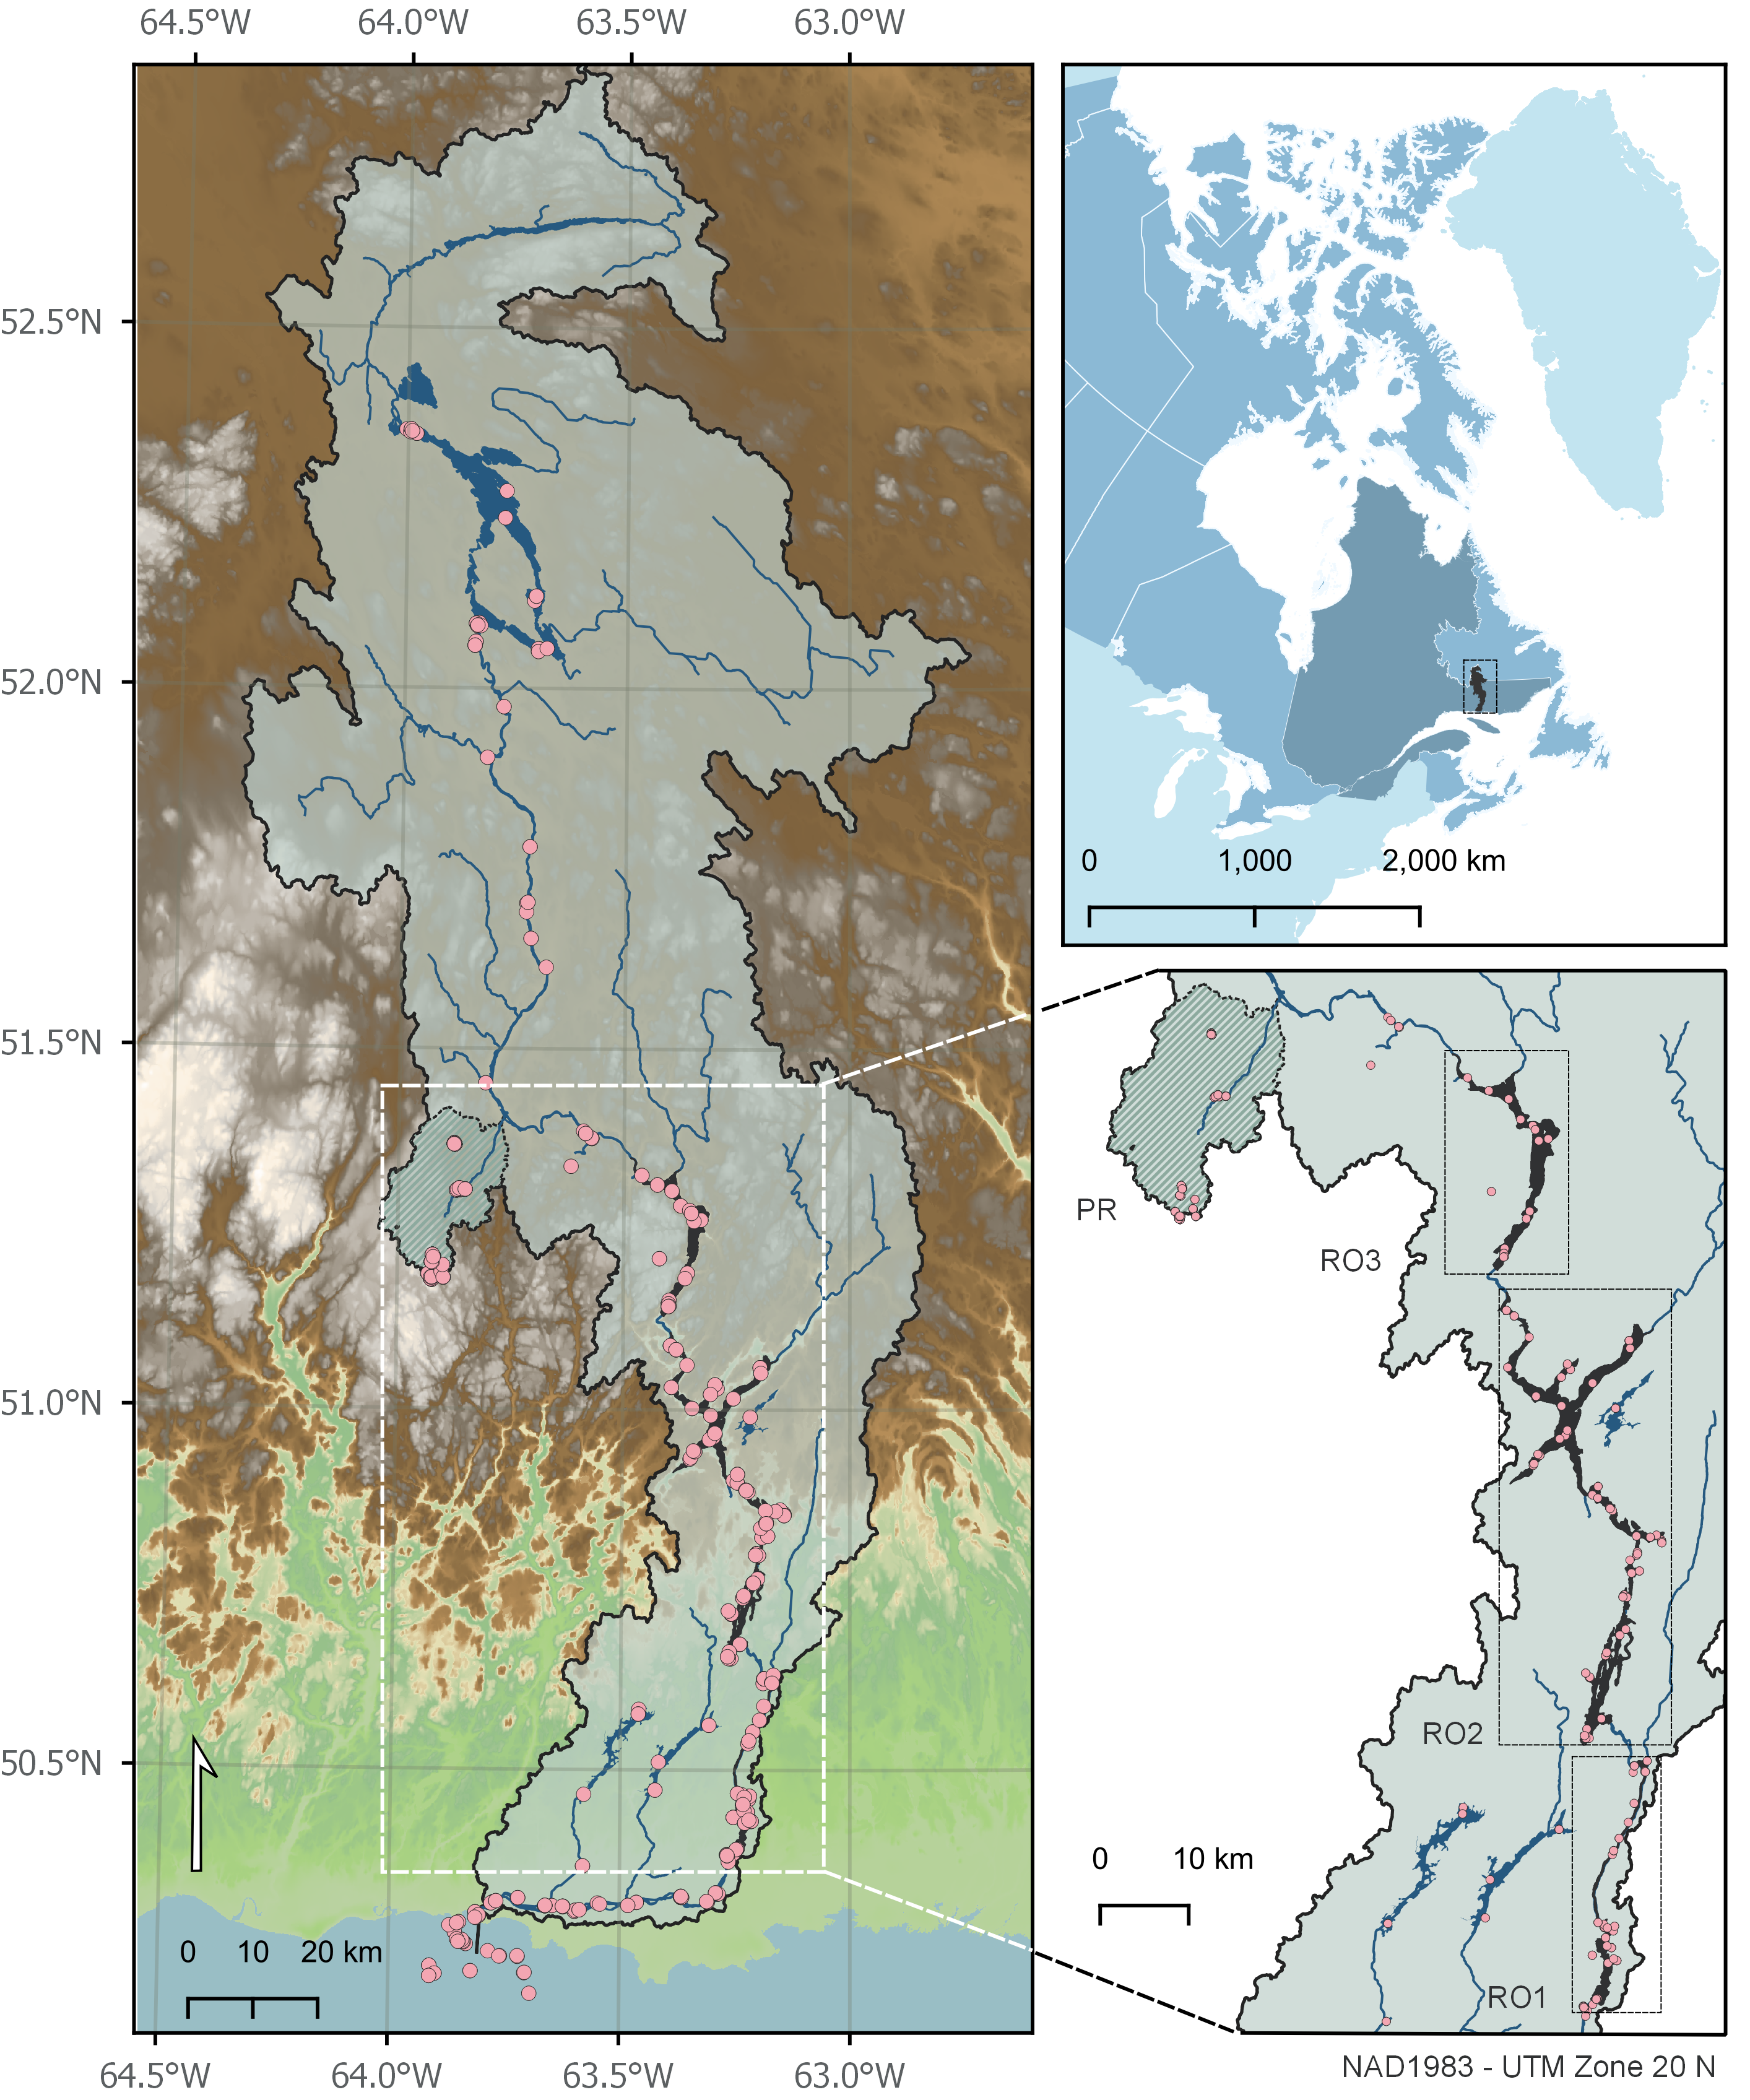
\includegraphics[width=12cm]{../Figures/LR_miccom_paper_threemaps.png}
\caption{\textbf{Location and overview of the La Romaine catchment}. a) Scale and overview of the whole La Romaine catchment. Samples are represented as points. b) Location of the catchment within Canada and Québec. c) Focus on all built reservoirs RO1 (2015), RO2 (2014) and RO3 (2017) and the headwater stream sub-catchment Petite Romaine (PR).}
%includegraphics[width=1\textwidth]
\end{figure}

\begin{figure}[!ht]
\centering
\includegraphics[width=15cm]{../../Figures/Final/PCoA_log_DNA_SampleType.png}
\caption{\textbf{Microbial community composition gradually changes along a terrestrial-hyrodlogical continuum and diverges between seasons.} PCoA analysis reveals microbial community shifts from terrestrial to freshwater samples. Spring and summer-autumn show distinct paths in multivariate space. Seasons are given in different point shapes, colouring visualises different habitat types. Percentage of variance explained are given in brackets for the first and second axis.}
%includegraphics[width=1\textwidth]
\end{figure}

\begin{figure}[!ht]
\centering
\includegraphics[width=17cm]{../../Figures/Final/PCoA_all_SampleType.png}
\caption{\textbf{RNA assemblages diverge from DNA within aquatic habitats, less so in terrestrially influenced habitats.} PCoA analysis inclduing RNA samples. a) Visualisation of first and second axis of PCoA, differentiating habitat type and nucleic acid type, respectively. b) Different view on PCoA analysis using the second and third axis, differentiating nucleic acid type and seasons, respectively. Seasons are given in different point shapes, colouring visualises different habitat types, opacity indicates nucleic acid type. Percentage of variance explained are given in brackets for the first, second and third axes.}
%includegraphics[width=1\textwidth]
\end{figure}



\end{document}
